\date{}
\title{}
\date{}
\usepackage{pgfplots}
\pgfplotsset{compat=1.14}
\begin{document}
\begin{frame}
    \titlepage
\end{frame}

\begin{frame}{last time}
    \begin{itemize}
    \item HTTP proxies
        \begin{itemize}
        \item forward, reverse
        \end{itemize}
    \item REST APIs
    \item passing values between servers
    \item multiaccess media
    \item (lack of) efficiency with collisions
        \begin{itemize}
        \item $\sim$18\% effective rate with no coordination
        \end{itemize}
    \item carrier sense idea
    \item slot-based retransmission
    \end{itemize}
\end{frame}

\begin{frame}[label=slotEx]{exercise: slots and variable packet size}
    \begin{itemize}
    \item say: packet time is 1$\mu s$ to 10$\mu s$
    \item say: minimum 0.1$\mu s$ to detect carrier
    \item use algorithm where we retransmit $K=rand(0, 32)$ slots after last transmission if there was contention
    \item what slot size to use?
    \end{itemize}
\end{frame}

\begin{frame}{multiple slots per transmission okay}
    % FIXME: diagram, to be added back to wireless
        % showing slots and multi-slot transmission
        % showing sense in slot before
\end{frame}

% FIXME: correction re: retransmission

\section{carrier-sense multiple access}
\begin{frame}{carrier sense}
    \begin{itemize}
    \item channel can be `busy' or not
    \item radio/light:
        \begin{itemize}
        \item have some sort of signal detectable on frequency
        \end{itemize}
    \vspace{.5cm}
    \item ``carrier sense''
    \item way to detect whether channel busy
    \end{itemize}
\end{frame}



\againframe<2>{slotEx}

\subsection{collision detection versus avoidance}
    % FIXME: diagram for ethernet collision detection + retransmit
\begin{frame}{collision detection}
    \begin{itemize}
    \item Wi-Fi: use ACKs to detect if transmission successful
    \item problem: transmit whole packet, then know about collision
    \vspace{.5cm}
    \item alternate idea: listen for collision, stop transmitting early
    \item doesn't work on wireless (we'll talk about why later)
    \item but does work on some wired shared media
    \item part of reason for design of Ethernet header
    \end{itemize}
\end{frame}

\usetikzlibrary{arrows.meta,shapes,shapes.misc}
\begin{frame}{collision detection takes time}
\begin{tikzpicture}[y=0.7cm]
\tikzset{
    wire/.style={draw,very thick,Circle-Circle},
    signal1/.style={draw,line width=1mm,red,-Latex},
    signal2/.style={draw,line width=2mm,dotted,violet,-Latex},
}
\draw[wire] (0, 0) -- (12, 0);
\draw[wire] (0, -1) -- (12, -1);
\draw[signal1] (0, -1) -- (2, -1);

\draw[wire] (0, -2) -- (12, -2);
\draw[signal1] (0, -2) -- (4, -2);
\draw[signal2] (12, -2) -- (10, -2);

\draw[wire] (0, -3) -- (12, -3);
\draw[signal1] (0, -3) -- (6, -3);
\draw[signal2] (12, -3) -- (8, -3);

\draw[wire] (0, -4) -- (12, -4);
\draw[signal1] (0, -4) -- (8, -4);
\draw[signal2] (12, -4) -- (6, -4);

\draw[wire] (0, -5) -- (12, -5);
\draw[signal1] (0, -5) -- (10, -5);
\draw[signal2] (12, -5) -- (4, -5);

\draw[wire] (0, -6) -- (12, -6);
\draw[signal1] (0, -6) -- (12, -6);
\draw[signal2] (12, -6) -- (2, -6);
\node[draw=red,line width=2mm,minimum width=.5cm,minimum height=.5cm,cross out] at (13, -6) {};

\draw[wire] (0, -7) -- (12, -7);
\draw[signal1] (0, -7) -- (12, -7);
\draw[signal2] (11, -7) -- (0, -7);
\node[draw=red,line width=2mm,minimum width=.5cm,minimum height=.5cm,cross out] at (-1, -7) {};

\draw[wire] (0, -8) -- (12, -8);
\draw[signal1] (2, -8) -- (12, -8);
\draw[signal2] (9, -8) -- (0, -8);
\end{tikzpicture}
\end{frame}

\begin{frame}{exercise: Ethernet cable length/delay}
    \begin{itemize}
    \item copper cable: about 2/3rds speed of light propogation
    \item 100Mbit ethernet has 64byte minimum frame size
    \vspace{.5cm}
    \item exercise: maximum cable length with collision detection?
    \end{itemize}
\end{frame}

\begin{frame}{solution}
\begin{tikzpicture}[y=0.7cm]
\tikzset{
    wire/.style={draw,very thick,Circle-Circle},
    signal1/.style={draw,line width=1mm,red,-Latex},
    signal2/.style={draw,line width=2mm,dotted,violet,-Latex},
}
\draw[wire] (0, -6) node[left]{A} -- (12, -6) node[right] {B};
\draw[signal1] (0, -6) -- (12, -6);
\draw[signal2] (12, -6) -- (1, -6);
\node[draw=red,line width=2mm,minimum width=.5cm,minimum height=.5cm,cross out] at (13, -6) {};
\end{tikzpicture}
\begin{itemize}
\item worst case: A and B maximally far apart on network and collide
    \begin{itemize}
    \item need each of them to detect collision and resend
    \item if they're maximum distance, then anyone else will get interference
    \end{itemize}
\item A transmits at time 0, takes $X$ time units to reach B
\item B transmits at time $X-\epsilon$, then detects collision
\item need A to also detect collision before it finishes sending frame
\item maximum packet length is how much we can send in $2X$ time units
\item 2X = 64 times 8 / 100Mbps  = 5.12 $\mu$ s; X = 2.56 $\mu$s
\end{itemize}
\end{frame}

\begin{frame}{propogation delay}
\begin{itemize}
\item transmission time for 64 bytes is 2.56 $\mu$s
\item propogation delay: approx 0.2 meters/ns or 200 meters/$\mu$s
\item 2.56 $\mu$s is about 512 meteres
\end{itemize}
\end{frame}




\section{wireless model, hidden and exposed nodes} 
    % FIXME: exposed nodes with walls
\begin{frame}{free space wireless transmission}
\begin{itemize}
\item assuming 2.4GHz Wifi, no obstacles, omnidirectional transmission:
\item 10 dB loss = $\frac{1}{10}$th power; 20 dB loss = $\frac{1}{100}$th power
\end{itemize}
\begin{tikzpicture}
\begin{axis}[
    xlabel={distance from transmitter (m)},
    ylabel={lost signal (dB)},
    width=12cm,
    height=5.5cm,
    xmode=log,
]
\addplot table {freespacemodel.table};
%\addplot[domain=0.1:100,samples=100] { 20*log(d/1000.0)/log(10) + 20*log(2.4)/log(10) + 92.45 };
\end{axis}
\end{tikzpicture}
\end{frame}


\begin{frame}{receiving multiple nodes}
\begin{tikzpicture}
\begin{pgfonlayer}{fg}
    \draw[fill=black] (0, 0) circle (.2cm)
        node[above=1mm] {D};
    \draw[fill=black] (2, -1) circle (.2cm)
        node[below=1mm] {A};
    \draw[fill=black] (12, 1) circle (.2cm)
        node[below=1mm] {B};
\end{pgfonlayer}
\tikzset{
    signal/.style={draw,violet,line width=1.4mm,-Latex},
    signal fade/.style={draw,violet!60!white,line width=.8mm},
    signal fade2/.style={draw,violet!30!white,line width=.4mm},
    signal end/.style={-{Latex[sep=0.2cm]}},
    signalB/.style={draw,blue,line width=1.4mm,-Latex},
    signal fadeB/.style={draw,blue!60!white,line width=.8mm},
    signal fade2B/.style={draw,blue!30!white,line width=.4mm},
}
\draw[signal,signal end] (2, -1) -- (0, 0);
\draw[signalB,-] (12, 1) -- (10, 10/12);
\draw[signal fadeB,-] (10, 10/12) -- (8, 8/12);
\draw[signal fade2B,signal end] (8, 8/12) -- (0, 0);
\end{tikzpicture}
\begin{itemize}
\item A's signal much much stronger at D
\item D may still receive A's signal\ldots
\item because B relatively too weak to interfere
\end{itemize}
\end{frame}

\begin{frame}{collision (non-)detection}
\begin{tikzpicture}
\begin{pgfonlayer}{fg}
    \draw[fill=black] (7, 0) circle (.2cm)
        node[above=1mm] {D};
    \draw[fill=black] (2, 1) circle (.2cm)
        node[below=1mm] {A};
    \draw[fill=black] (12, 1) circle (.2cm)
        node[below=1mm] {B};
\end{pgfonlayer}
\tikzset{
    signal/.style={draw,violet,line width=1.4mm,-Latex},
    signal fade/.style={draw,violet!60!white,line width=.8mm},
    signal fade2/.style={draw,violet!30!white,line width=.4mm},
    signal end/.style={-{Latex[sep=0.2cm]}},
    signalB/.style={draw,blue,line width=1.4mm,-Latex},
    signal fadeB/.style={draw,blue!60!white,line width=.8mm},
    signal fade2B/.style={draw,blue!30!white,line width=.4mm},
}
\draw[signal,-] (2, 1) -- (4, 3/5);
\draw[signal fade,signal end] (4, 3/5) -- (7, 0);
\draw[signalB,-] (12, 1) -- (10, 3/5);
\draw[signal fadeB,signal end] (10, 3/5) -- (7, 0);'
\begin{visibleenv}<1>
    \node[anchor=north,draw=red,align=left,very thick] at (7, -0.2) {
        D receives junk
    };
\end{visibleenv}
\begin{visibleenv}<2>
\draw[signal,-] (2, 1) -- (4.5, 1);
\draw[signal fade,-] (4.5, 1) -- (7, 1);
\draw[signal fade2,signal end] (7, 1) -- (12, 1);
\draw[red,very thick] (12, 1) circle (.3cm);
    \node[anchor=north,draw=red,align=left,very thick] at (12, 0.2) {
        B's own transmission\\
        is much stronger than A's \\
        cannot detect collision itself
    };
\end{visibleenv}
\end{tikzpicture}
\end{frame}

\begin{frame}{carrier-sense}
\begin{tikzpicture}
\begin{pgfonlayer}{fg}
    \draw[fill=black] (7, 0) circle (.2cm)
        node[above=1mm] {D};
    \draw[fill=black] (2, 1) circle (.2cm)
        node[below=1mm] {A};
    \draw[fill=black] (12, 1) circle (.2cm)
        node[below=1mm] {B};
\end{pgfonlayer}
\tikzset{
    signal/.style={draw,violet,line width=1.4mm,-Latex},
    signal fade/.style={draw,violet!60!white,line width=.8mm},
    signal fade2/.style={draw,violet!30!white,line width=.4mm},
    signal end/.style={-{Latex[sep=0.2cm]}},
}
\draw[signal,-] (2, 1) -- (4, 3/5);
\draw[signal fade,signal end] (4, 3/5) -- (7, 0);
\draw[signal,-] (2, 1) -- (4.5, 1);
\draw[signal fade,-] (4.5, 1) -- (7, 1);
\draw[signal fade2,signal end] (7, 1) -- (12, 1);
\draw[red,very thick] (12, 1) circle (.3cm);
    \node[anchor=north,draw=red,align=left,very thick] at (12, 0.2) {
        B can detect A's transmitting \\
        avoid starting transmission now
    };
\end{tikzpicture}
\end{frame}

\begin{frame}{carrier-not-sensing}
\begin{tikzpicture}
\begin{pgfonlayer}{fg}
    \draw[fill=black] (7, 0) circle (.2cm)
        node[above=1mm] {D};
    \draw[fill=black] (2, 1) circle (.2cm)
        node[below=1mm] {A};
    \draw[fill=black] (14, 1) circle (.2cm)
        node[below=1mm] {B};
\end{pgfonlayer}
\tikzset{
    signal/.style={draw,violet,line width=1.4mm,-Latex},
    signal fade/.style={draw,violet!60!white,line width=.8mm},
    signal fade2/.style={draw,violet!30!white,line width=.4mm},
    signal fade3/.style={draw,violet!15!white,line width=.2mm},
    signal end/.style={-{Latex[sep=0.2cm]}},
    range mark/.style={draw,violet!50!black,dotted,line width=1mm},
}
\begin{scope}
    \clip (1, -6) rectangle (15, 2);
    \draw[overlay,range mark,fill=violet!10] (2, 1) circle (10.5 cm);
        \node[font=\Huge] at (4, -2) {A's range};
\end{scope}
\draw[signal,-] (2, 1) -- (4, 3/5);
\draw[signal fade,signal end] (4, 3/5) -- (7, 0);
\draw[signal,-] (2, 1) -- (4.5, 1);
\draw[signal fade,-] (4.5, 1) -- (7, 1);
\draw[signal fade2,-] (7, 1) -- (9, 1);
\draw[signal fade3,signal end] (9, 1) -- (12.5, 1);
\draw[red,very thick] (14, 1) circle (.3cm);
    \node[anchor=north,draw=red,align=left,very thick,fill=white] at (14, 0.2) {
        B doesn't know \\ A is transmitting \\
        because A's signal\\
        is too weak
    };
\end{tikzpicture}
\end{frame}

\begin{frame}{`hidden node' problem}
\begin{tikzpicture}
\begin{pgfonlayer}{fg}
    \draw[fill=black] (4, 0) circle (.2cm)
        node[above=1mm] {D};
    \draw[fill=black] (2, 1) circle (.2cm)
        node[below=1mm] {A};
    \draw[fill=black] (6, 0.5) circle (.2cm)
        node[below=1mm] {B};
\end{pgfonlayer}
\tikzset{
    signal/.style={draw,violet,line width=1.4mm,-Latex},
    signalB/.style={draw,blue,line width=1.4mm,-Latex},
    signal fade/.style={draw,violet!60!white,line width=.8mm},
    signal fade2/.style={draw,violet!30!white,line width=.4mm},
    signal fade3/.style={draw,violet!15!white,line width=.2mm},
    signal end/.style={-{Latex[sep=0.2cm]}},
    range mark/.style={draw,violet!50!black,dotted,line width=1mm},
    range markB/.style={draw,blue!50!black,dashed,line width=1mm},
}
\draw[signal,signal end] (2, 1) -- (4,0);
\draw[signalB,signal end] (6, .5) -- (4,0);
\begin{scope}
    \clip (-1, -6) rectangle (15, 2);
    \draw[overlay,range mark] (2, 1) circle (3.5 cm);
    \draw[overlay,range markB] (6, 0.5) circle (3.5 cm);
\end{scope}
\end{tikzpicture}
\begin{itemize}
\item B is a `hidden node' for A and vice-versa
\end{itemize}
\end{frame}

\begin{frame}{carrier false sensing}
\begin{tikzpicture}
\begin{pgfonlayer}{fg}
    \draw[fill=black] (4, 1) circle (.2cm)
        node[below=1mm] {A};
    \draw[fill=black] (1, -1) circle (.2cm)
        node[below=1mm] {C};
    \draw[fill=black] (9, 1) circle (.2cm)
        node[below=1mm] {B};
    \draw[fill=black] (12, 1) circle (.2cm)
        node[below=1mm] {D};
\end{pgfonlayer}
\tikzset{
    signal/.style={draw,violet,line width=1.4mm,-Latex},
    signal fade/.style={draw,violet!60!white,line width=.8mm},
    signal fade2/.style={draw,violet!30!white,line width=.4mm},
    signal fade3/.style={draw,violet!15!white,line width=.2mm},
    signal end/.style={-{Latex[sep=0.2cm]}},
    signalB/.style={draw,blue,line width=1.4mm,-Latex},
    signal fadeB/.style={draw,blue!60!white,line width=.8mm},
    signal fade2B/.style={draw,blue!30!white,line width=.4mm},
    range mark/.style={draw,violet!50!black,dotted,line width=1mm},
    range markB/.style={draw,blue!50!black,dashed,line width=1mm},
}
\draw[signal,signal end] (4, 1) -- (1, -1);
\begin{visibleenv}<1>
\draw[signalB,signal end] (9, 1) -- (12, 1);
\end{visibleenv}
\begin{visibleenv}<2>
\draw[signal fade,signal end] (4, 1) -- (9, 1);
\end{visibleenv}
\begin{scope}
    \clip (1, -6) rectangle (15, 2);
    \draw[overlay,range mark] (4, 1) circle (6cm);
    \draw[overlay,range markB] (9, 1) circle (6cm);
\end{scope}
\begin{visibleenv}<1>
    \node[align=left,anchor=north,red,very thick] at (6, -.5) {
        A$\rightarrow$C and B$\rightarrow$D won't collide! \\
    };
\end{visibleenv}
\begin{visibleenv}<2>
    \node[align=left,anchor=north,red,very thick,fill=white,draw=red] at (6, -.5) {
        B will detect carrier \\
        may avoid transmitting to D \\
        even though there is no interference!
    };
\end{visibleenv}
\end{tikzpicture}
\end{frame}


\begin{frame}{hidden/exposed node summary}
\begin{tikzpicture}
\begin{scope}[x=0.3cm,y=0.5cm]
    \begin{pgfonlayer}{fg}
        \draw[fill=black] (4, 1) circle (.2cm)
            node[below=1mm] {A};
        \draw[fill=black] (1, -1) circle (.2cm)
            node[below=1mm] {C};
        \draw[fill=black] (9, 1) circle (.2cm)
            node[below=1mm] {B};
        \draw[fill=black] (12, 1) circle (.2cm)
            node[below=1mm] {D};
    \end{pgfonlayer}
    \tikzset{
        signal/.style={draw,violet,line width=1.4mm,-Latex},
        signal fade/.style={draw,violet!60!white,line width=.8mm},
        signal fade2/.style={draw,violet!30!white,line width=.4mm},
        signal fade3/.style={draw,violet!15!white,line width=.2mm},
        signal end/.style={-{Latex[sep=0.2cm]}},
        signalB/.style={draw,blue,line width=1.4mm,-Latex},
        signal fadeB/.style={draw,blue!60!white,line width=.8mm},
        signal fade2B/.style={draw,blue!30!white,line width=.4mm},
        range mark/.style={draw,violet!50!black,dotted,line width=.4mm},
        range markB/.style={draw,blue!50!black,dashed,line width=.4mm},
    }
    \draw[violet,dotted,very thick,signal end] (4, 1) -- (1, -1);
    \draw[blue,dotted,very thick,signal end] (9, 1) -- (12, 1);
    \begin{scope}
        \clip (-5, -5) rectangle (20, 4);
        \draw[overlay,range mark] (4, 1) circle (2cm);
        \draw[overlay,range markB] (9, 1) circle (2cm);
    \end{scope}
    \node[anchor=west,align=left,font=\small] at (18, 0) {
        \textit{exposed node problem}: A and B \\
        detect each other's transmissions \\
        but don't interfere 
    };
\end{scope}
\begin{scope}[yshift=-4cm,x=0.3cm,y=0.5cm]
    \begin{pgfonlayer}{fg}
        \draw[fill=black] (1, 1) circle (.2cm)
            node[below=1mm] {A};
        \draw[fill=black] (4, -1) circle (.2cm)
            node[below=1mm] {C};
        \draw[fill=black] (8, -1) circle (.2cm)
            node[below=1mm] {B};
    \end{pgfonlayer}
    \tikzset{
        signal/.style={draw,violet,line width=1.4mm,-Latex},
        signal fade/.style={draw,violet!60!white,line width=.8mm},
        signal fade2/.style={draw,violet!30!white,line width=.4mm},
        signal fade3/.style={draw,violet!15!white,line width=.2mm},
        signal end/.style={-{Latex[sep=0.2cm]}},
        signalB/.style={draw,blue,line width=1.4mm,-Latex},
        signal fadeB/.style={draw,blue!60!white,line width=.8mm},
        signal fade2B/.style={draw,blue!30!white,line width=.4mm},
        range mark/.style={draw,violet!50!black,dotted,line width=.4mm},
        range markB/.style={draw,blue!50!black,dashed,line width=.4mm},
    }
    \begin{scope}
        \clip (-1, -5) rectangle (15, 4);
        \draw[overlay,range mark] (0, 1) circle (2cm);
        \draw[overlay,range markB] (8, -1) circle (2cm);
    \end{scope}
    \draw[violet,dotted,very thick,signal end] (1, 1) -- (4, -1);
    \draw[blue,dotted,very thick,signal end] (8, -1) -- (4, -1);
    \node[anchor=west,align=left,font=\small] at (18, 0) {
        \textit{hidden node problem}: A and B interfere \\
        when sending to C\\
        but can't detect each other's transmissions
    };
\end{scope}
\end{tikzpicture}
\end{frame}


\section{RTS/CTS}

\begin{frame}{ready-to-send/clear-to-send}
    \begin{itemize}
    \item can't detect likely interference at sender
    \item but can at receiver
    \vspace{.5cm}
    \item idea: have receiver tell when it's okay to transmit
    \end{itemize}
\end{frame}


\subsection{RTS/CTS exercise}
\begin{frame}{exercise: RTS/CTS suitablity}
    \begin{itemize}
    \item RTS/CTS is a better idea when\ldots?
    \item A. almost all messages are sent by one node instead of being split evenly
    \item B. messages are shorter 
    \item D. more nodes can hear others who are transmitting to different base stations
    \item C. more nodes cannot hear others who are transmitting to the same base station
    \end{itemize}
\end{frame}


\section{multipath}

\begin{frame}{multipath interference}
\begin{tikzpicture}
\begin{pgfonlayer}{fg}
    \draw[fill=black] (0, 0) circle (.2cm);
    \draw[fill=black] (12, -4) circle (.2cm);
    \begin{scope}[ultra thick]
        \draw (-2, 2) rectangle (13, -5);
    \end{scope}
\end{pgfonlayer}
\tikzset{
    signal/.style={draw,violet,line width=.8mm,-Latex},
    signal fade/.style={draw,violet!60!white,line width=.8mm},
    signal fade2/.style={draw,violet!30!white,line width=.8mm},
    signal end/.style={-{Latex[sep=0.2cm]}},
}
\draw[signal] (0, 0) -- (12 / 3, 6 / 3);
\draw[signal fade,signal end] (12 / 3, 6 / 3) -- (12, -4);
\draw[signal] (0, 0) -- (-14 / 7, -4 / 7);
\draw[signal fade,signal end] (-14 / 7, -4 / 7) -- (12, -4);
\draw[signal] (0, 0) -- (14 * 13 / 14, -4 * 13 / 14);
\draw[signal fade, signal end] (14 * 13 / 14, -4 * 13 / 14) -- (12, -4);
\draw[signal] (0, 0) -- (14 * 5 / 6, -6 * 5 / 6);
\draw[signal fade, signal end] (14 * 5 / 6, -6 * 5 / 6) -- (12, -4);

\draw[signal,signal end] (0, 0) -- (12, -4);
\end{tikzpicture}
\end{frame}

\begin{frame}{simple self-interference}
\begin{tikzpicture}
\begin{axis}[name=top1,hide axis,width=7cm,height=4cm,ymin=-1,ymax=1]
    \addplot[domain=0:1000,samples=1000] {sin(x*4) * sin(0.75+x/3)};
    \coordinate (top1 tl) at (axis cs:0, 1);
    \coordinate (top1 br) at (axis cs:1000, -1);
\end{axis}
\coordinate (middle base) at ([yshift=-2cm]top1.east);
\coordinate (low base) at ([yshift=-4cm]top1.east);
\begin{axis}[anchor=east,name=middle1,at={(middle base)},width=7cm,height=4cm,hide axis,
    ymin=-1,ymax=1]
    \addplot[domain=0:1000,samples=1000] {0.4*(sin((x+45)*4) * sin(0.75+(x + 45)/3))};
    \coordinate (middle1 tl) at (axis cs:0, 0.4);
    \coordinate (middle1 br) at (axis cs:1000, -0.4);
\end{axis}
\begin{axis}[hide axis,width=7cm,height=4cm,anchor=east,name=combine1,at={(low base)},
    ymin=-1,ymax=1]
    \addplot[domain=0:1000,samples=1000] {
     sin(x*4) * sin(0.75+x/3) +
     0.5*(sin((x+45)*4) * sin(0.75+(x + 45)/3))
    };
\end{axis}
\coordinate (top2 base) at ([xshift=2cm]top1.east);
\begin{axis}[anchor=west,at={(top2 base)},name=top2,hide axis,width=7cm,height=4cm,ymin=-1,ymax=1]
    \addplot[domain=0:1000,samples=1000] {sin(x*4) * sin(0.75+x/3)};
    \coordinate (top2 tl) at (axis cs:0, 1);
    \coordinate (top2 br) at (axis cs:1000, -1);
\end{axis}
\coordinate (middle base2) at ([yshift=-2cm]top2.east);
\coordinate (low base2) at ([yshift=-4cm]top2.east);
\begin{axis}[anchor=east,name=middle2,at={(middle base2)},width=7cm,height=4cm,hide axis,
    ymin=-1,ymax=1]
    \addplot[domain=0:1000,samples=1000] {0.4*(sin((x+25)*4) * sin(0.75+(x + 25)/3))};
    \coordinate (middle2 tl) at (axis cs:0, 0.4);
    \coordinate (middle2 br) at (axis cs:1000, -0.4);
\end{axis}
\begin{axis}[hide axis,width=7cm,height=4cm,anchor=east,name=combine2,at={(low base2)},
    ymin=-1,ymax=1]
    \addplot[domain=0:1000,samples=1000] {
     sin(x*4) * sin(0.75+x/3) +
     0.5*(sin((x+25)*4) * sin(0.75+(x + 25)/3))
    };
\end{axis}
\node[font=\large]  at (middle1.west) {+};
\node[font=\large]  at (middle2.west) {+};
\draw[ultra thick] (middle1.south west) -- (middle1.south east);
\draw[ultra thick] (middle2.south west) -- (middle2.south east);
\begin{visibleenv}<2>
\draw[very thick,red] (top1 tl) rectangle (top1 br);
\draw[very thick,red] (top2 tl) rectangle (top2 br);
\node[font=\small,anchor=west,red] at (top1.east) {original};
\draw[very thick,blue] (middle1 tl) rectangle (middle1 br);
\draw[very thick,blue] (middle2 tl) rectangle (middle2 br);
\node[font=\small,anchor=west,blue] at (middle1.east) {reflected};
\end{visibleenv}
\end{tikzpicture}
\end{frame}


\begin{frame}{multipath interference}
    \begin{itemize}
    \item quite complicated to predict in three dimensions, variable reflectivity, \ldots
    \item varies on frequency
        \begin{itemize}
        \item switching to close different channel may change a lot
        \end{itemize}
    \item can help and hurt signal reception
    \item especially bad when `inter-symbol interference'
        \begin{itemize}
        \item can be mitigated some by choice of message encoding
        \end{itemize}
    \vspace{.5cm}
    \item contributes to irregular `dead zones', etc.
    \end{itemize}
\end{frame}

\begin{frame}{deliberate multipath / MIMO}
    \begin{itemize}
    \item can have:
    \item multiple sending antennas (inputs) (MI)
    \item multiple receiving antennas (outputs) (MO)
    \item some simple ideas:
    \vspace{.5cm}
    \item receive signal twice, hope one antenna not in dead zone
    \item send signal twice, have receiver tell you which is better
    \end{itemize}
\end{frame}

\begin{frame}{multiple spatial streams}
\begin{tikzpicture}
\begin{scope}[every path/.style={fill=black!50,draw=black!50,text=black}]
    \path (-.5, .5) rectangle ++(.5, -4) node[midway] {A};
    \path (12, .5) -- (12.5, 0.3) -- (11.5, -3.5) -- (11, -3.3) -- cycle;
    \node at (11.7, -1.5) {B};
    \path (0, 0) circle (2mm) coordinate (A1) node[above right=1mm]{$A_1$};
    \path (0, -3) circle (2mm) coordinate (A2) node[below right=1mm]{$A_2$};
    \path (11.7, 0) circle (2mm) coordinate (B1) node[above left=1mm]{$B_1$};
    \path (11, -3) circle (2mm) coordinate (B2) node[below left=1mm]{$B_2$};
\end{scope}
\tikzset{
    strong/.style={line width=1.2mm,arrows={{Butt Cap[sep=5mm]}-{Latex[sep=5mm]}}},
    stronger/.style={line width=1.3mm,arrows={{Butt Cap[sep=5mm]}-{Latex[sep=5mm]}}},
    medium/.style={line width=1mm,arrows={{Butt Cap[sep=5mm]}-{Latex[sep=5mm]}}},
    weak/.style={line width=0.8mm,arrows={{Butt Cap[sep=5mm]}-{Latex[sep=5mm]}}},
}
\foreach \x/\y/\lw in {A1/B1/strong,A2/B2/stronger,A1/B2/medium,A2/B1/weak} {
    \draw[\lw] (\x) -- (\y);
}
\end{tikzpicture}
\begin{itemize}
\item<2-> signals might mix based on relative strengths, say
\begin{align*}
B_1 &\sim& 0.9A_1 &+& 0.7A_2 \\
B_2 &\sim& A_1 &+& 1.2A_2 
\end{align*}
\end{itemize}
\end{frame}

\begin{frame}{simplified multipath model}
\begin{align*}
B_1 &\sim& 0.9A_1 &+& 0.7A_2 \\
B_2 &\sim& A_1 &+& 1.2A_2 
\end{align*}
\begin{itemize}
\item if we can estimate coefficients\ldots
\item B can solve for $A_1$, $A_2$
\vspace{.5cm}
\item A can send with pattern to help estimate coefficients:
    \begin{itemize}
    \item example: send full power from $A_1$ ($(B_1,B_2)=(0.9, 1)$), then from $A_2$ ($(B_1,B_2)=(0.7, 1.2)$)
    \end{itemize}
\end{itemize}
\end{frame}

\begin{frame}{correlation problem}
    \begin{itemize}
    \item when two `spatial streams' correlated, harder to solve for them
    \item example: suppose $(B_1,B_2)=(A_1+A_2,A_1+1.1A_2)$
    \vspace{.5cm}
    \item $A_2=10B_1-10B_2$
    \item need 10x precision in $B_1$, $B_2$ to get 1x precision in $A_2$
    \end{itemize}
\end{frame}


% FIXME: short interframe spacing

\section{aside: assignment}
\begin{frame}{assignment}
    \begin{itemize}
    \item upcoming wireless assignment
    \item one receiver, many senders
    \item free space model (no multipath)
    \item can only change senders:
        \begin{itemize}
        \item get channel sense/ACK info
        \item choose channel
        \item choose timing of transmissions
        \end{itemize}
    \end{itemize}
\end{frame}

\section{ad-hoc v base stations}
\begin{frame}{wifi modes}
    \begin{itemize}
    \item ``ad-hoc'': everyone sends/receives from whoever
    \item ``infrastructure'': designated \textit{access points}
    \vspace{.5cm}
    \item mostly use infrastructure networks
    \end{itemize}
\end{frame}

\begin{frame}{infrastructure mode}
    \begin{itemize}
    \item networks identified by SSID (Service Set IDentifier)
        \begin{itemize}
        \item human readable name
        \end{itemize}
    \item single SSID can have many access points (example: eduroam)
    \item clients \textit{associated} with one access point at a time
    \vspace{.5cm}
    \item clients only \textit{only} send to their current access point
    \item \ldots even if sending to other nodes on network
    \end{itemize}
\end{frame}

\begin{frame}{exercise: why through AP?}
    \begin{itemize}
    \item case where going through AP helps performance?
    \item case where going through AP hurts performance?
    \end{itemize}
\end{frame}

\begin{frame}{beacons (approx. once per 100ms)}
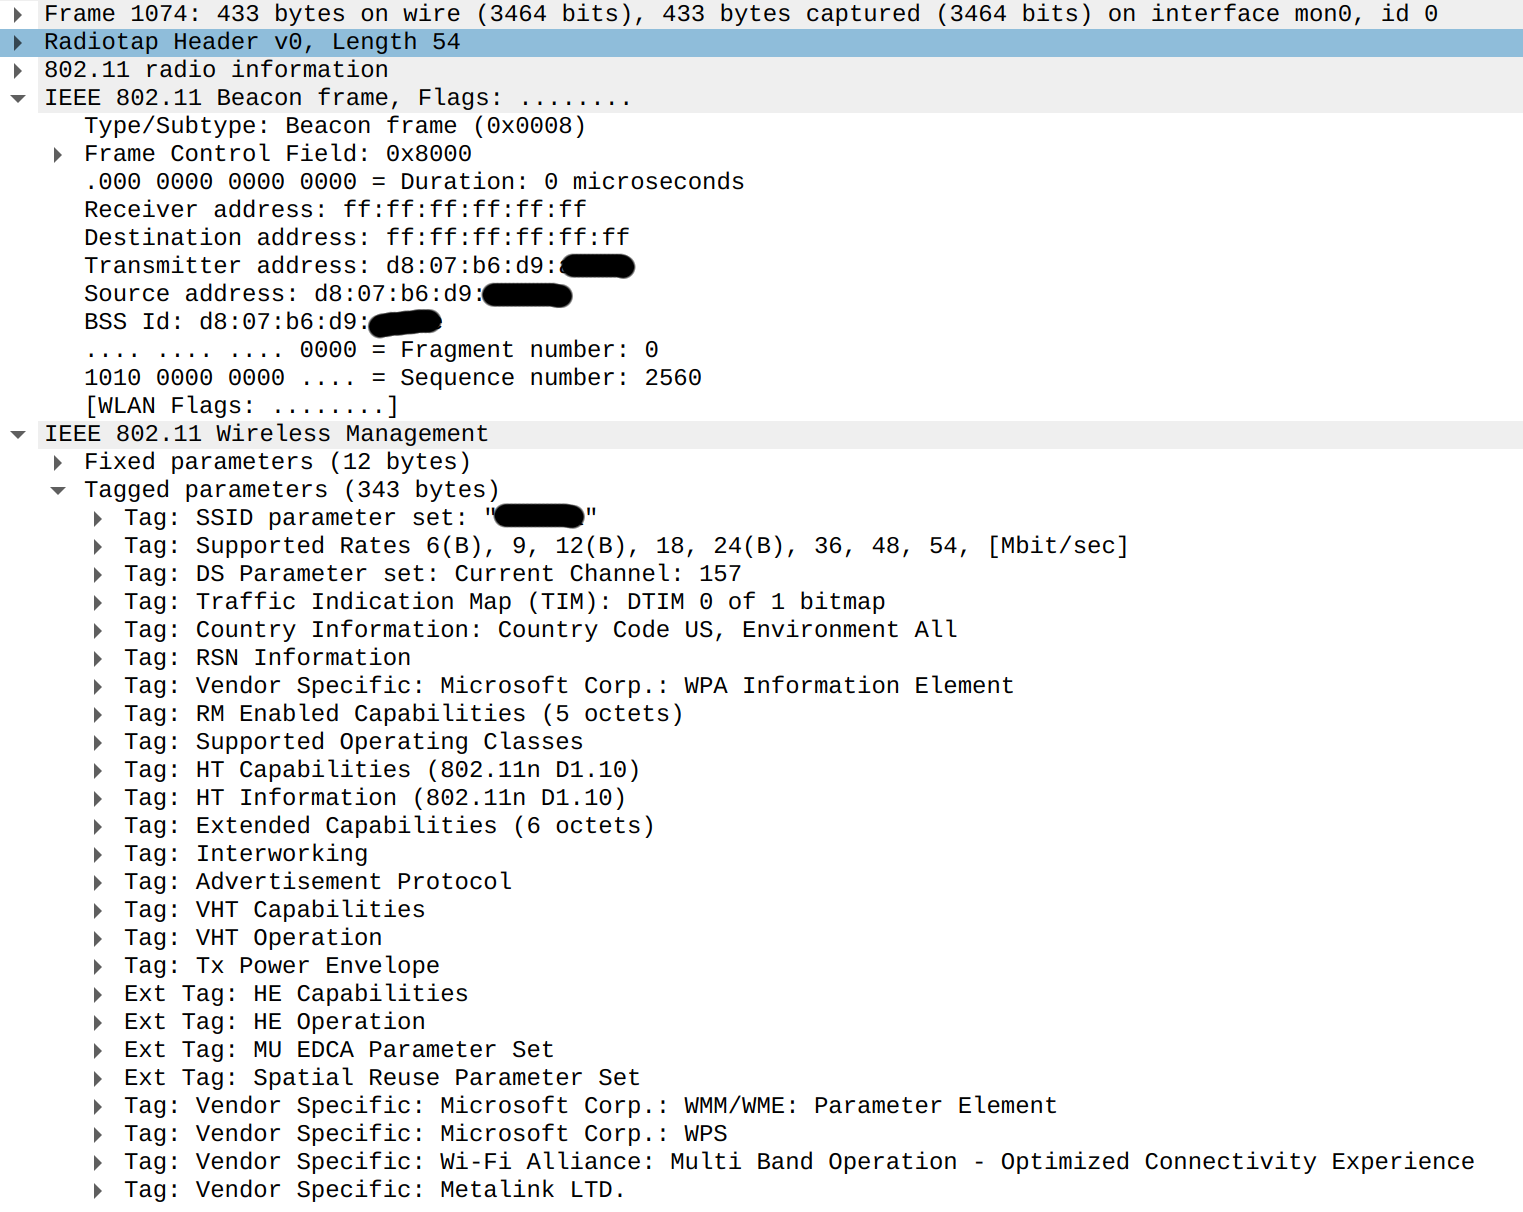
\includegraphics[height=0.85\textheight]{../multiaccess/wifi-beacon-1.png}
\end{frame}

\begin{frame}{probes/probe responses}
    \begin{itemize}
    \item beacons --- listen for a few seconds, find out about nearby networks
    \item probably need to scan multiple channels
    \vspace{.5cm}
    \item can also send explicit probes to learn about networks
    \item receive responses, with essentially same kind of information
    \end{itemize}
\end{frame}

\begin{frame}{association}
    \begin{itemize}
    \item client $\rightarrow$ AP: association response (SSID=\ldots)
    \item AP $\rightarrow$ client: association response (SSID=\ldots)
    \item + things related to WiFi Security (encryption, passwords, etc.)
    \vspace{.5cm}
    \item client $\rightarrow$ AP: deassociation (sometimes)
    \end{itemize}
\end{frame}

\begin{frame}{moving between APs}
    \begin{itemize}
    \item multiple APs can broadcast have same SSID
    \item generally: nodes should listen for beacons, measure signal-to-noise ratio
    \vspace{.5cm}
    \item eventually decide to change association
    \end{itemize}
\end{frame}


\begin{frame}{wifi data frames}
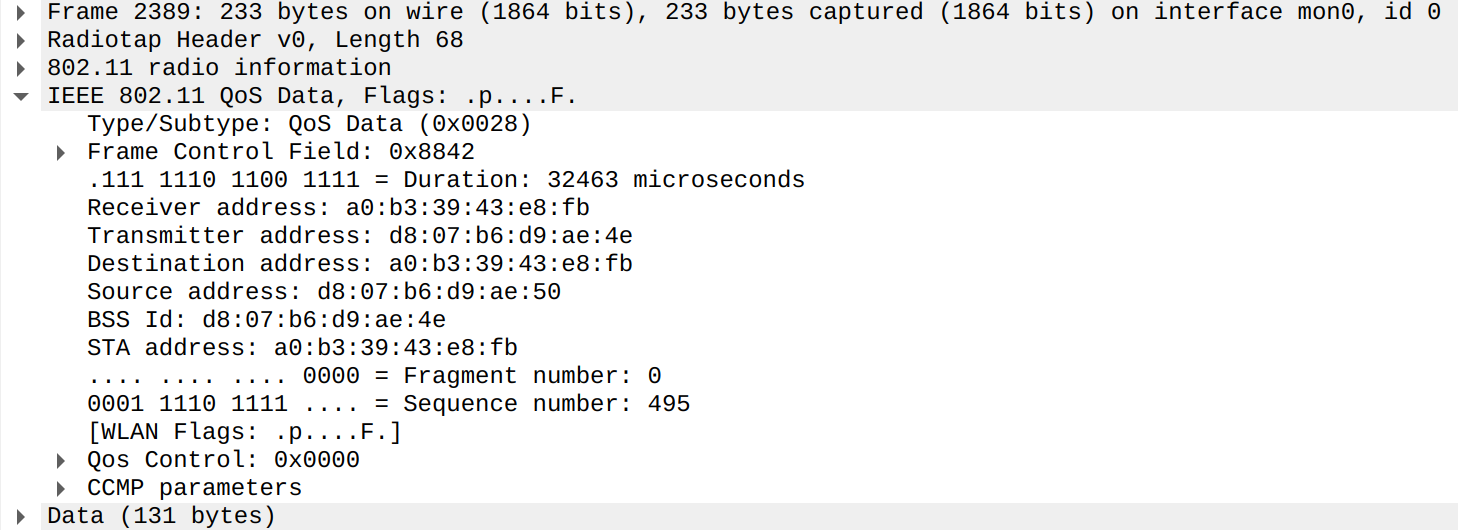
\includegraphics[height=0.85\textheight]{../multiaccess/wifi-data-1.png}
\end{frame}

\begin{frame}{wifi data}
\begin{tikzpicture}
\node (A) at (0, 0) {A};
\node (ap1) at (4, 0) {AP1};
\node (ap2) at (8, 0) {AP2};
\node (B) at (12, 0) {B};
\begin{scope}[-Latex]
\draw (A) -- (ap1);
\draw (ap1) -- (ap2);
\draw (ap2) -- (B);
\end{scope}
\end{tikzpicture}
    \begin{itemize}
    \item receiver/transmitter address --- this hop
    \item source/destination address --- final soruce/destination
    \vspace{.5cm}
    \item can differ if\ldots
        \begin{itemize}
        \item destination is a broadcast/multicast address
        \item wireless equivalent of `switching'
        \end{itemize}
    \end{itemize}
\end{frame}



\subsection{mobility}
\usetikzlibrary{calc}
\begin{frame}{multiple APs, one network}
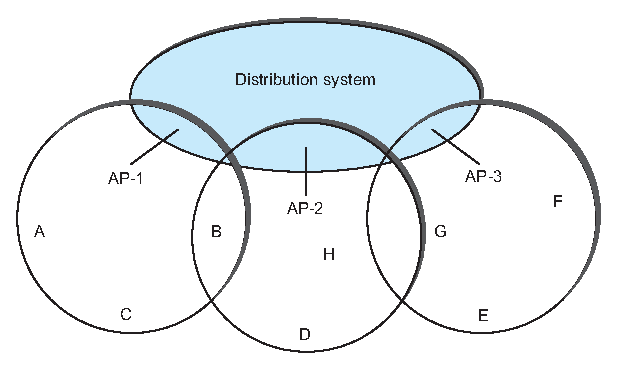
\includegraphics[width=\textwidth]{../multiaccess/cnsp-fig48}
\imagecredit{Computer Networks: A Systems Approach, figure 48}
\end{frame}

\begin{frame}{APs as switches}
    \begin{itemize}
    \item multiple APs can act as \textit{one network}
    \item example: nodes connected to different APs can send packets to each other by MAC address
    \vspace{.5cm}
    \item distribution system needs to share neighbor-table-like information
    \end{itemize}
\end{frame}

\begin{frame}{switching APs}
    \begin{itemize}
    \item nodes can switch APs\ldots
    \vspace{.5cm}
    \item check for new APs when signal strength too low
    \item periodically check for beacons + signal strength
    \vspace{.5cm}
    \item switching APs = same as joining network, but\ldots
        \begin{itemize}
        \item can keep IP address, etc.
        \item maybe optimizations to avoid redoing wifi security, etc.
        \end{itemize}
    \end{itemize}
\end{frame}

\begin{frame}{cellular networks}
    \begin{itemize}
    \item for wifi networks, feasible to track device locations centrally mostly
    \vspace{.5cm}
    \item need/have something more complex for cellular networks
    \end{itemize}
\end{frame}

\begin{frame}{a confusing picture}
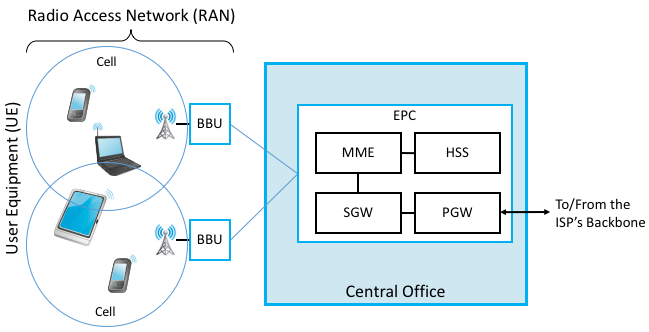
\includegraphics[width=\textwidth]{../multiaccess/sysapp-fig53}
\end{frame}

\begin{frame}{cellular mobility model}
    \begin{itemize}
    \item cellular networks: base stations don't know how to route to each end-host in whole cell network
    \vspace{.5cm}
    \item cell phone (UE) $\rightarrow$ base station (BBU) $\rightarrow$ service gateway (SGW) $\rightarrow$ PDN gateway (PGW)
    \vspace{.5cm}
    \item central `mobility management entity' (MME) sets up `tunnels' for steps above
        \begin{itemize}
        \item coordinates with home subscriber server (HSS)
        \item base stations don't track full routing information
        \end{itemize}
    \item PDN gateway stays stable so IP address can stay the same
        \begin{itemize}
        \item PDN gateway = gateway to actual Internet
        \end{itemize}
    \item in `roaming' situation:
        \begin{itemize}
        \item service gateway run by network you're connected to
        \item PDN gateway run by `home' network
        \end{itemize}
    \end{itemize}
\end{frame}



\subsection{mesh networks}
\begin{frame}{Roofnet (Cambridge, MA, 2005)}
{\fontsize{9}{10}\selectfont Bicket, Aguayo, Biswas, Morris, ``Architecture and Evaluation of
an Unplanned 802.11b Mesh Network (MobiCom'05)}
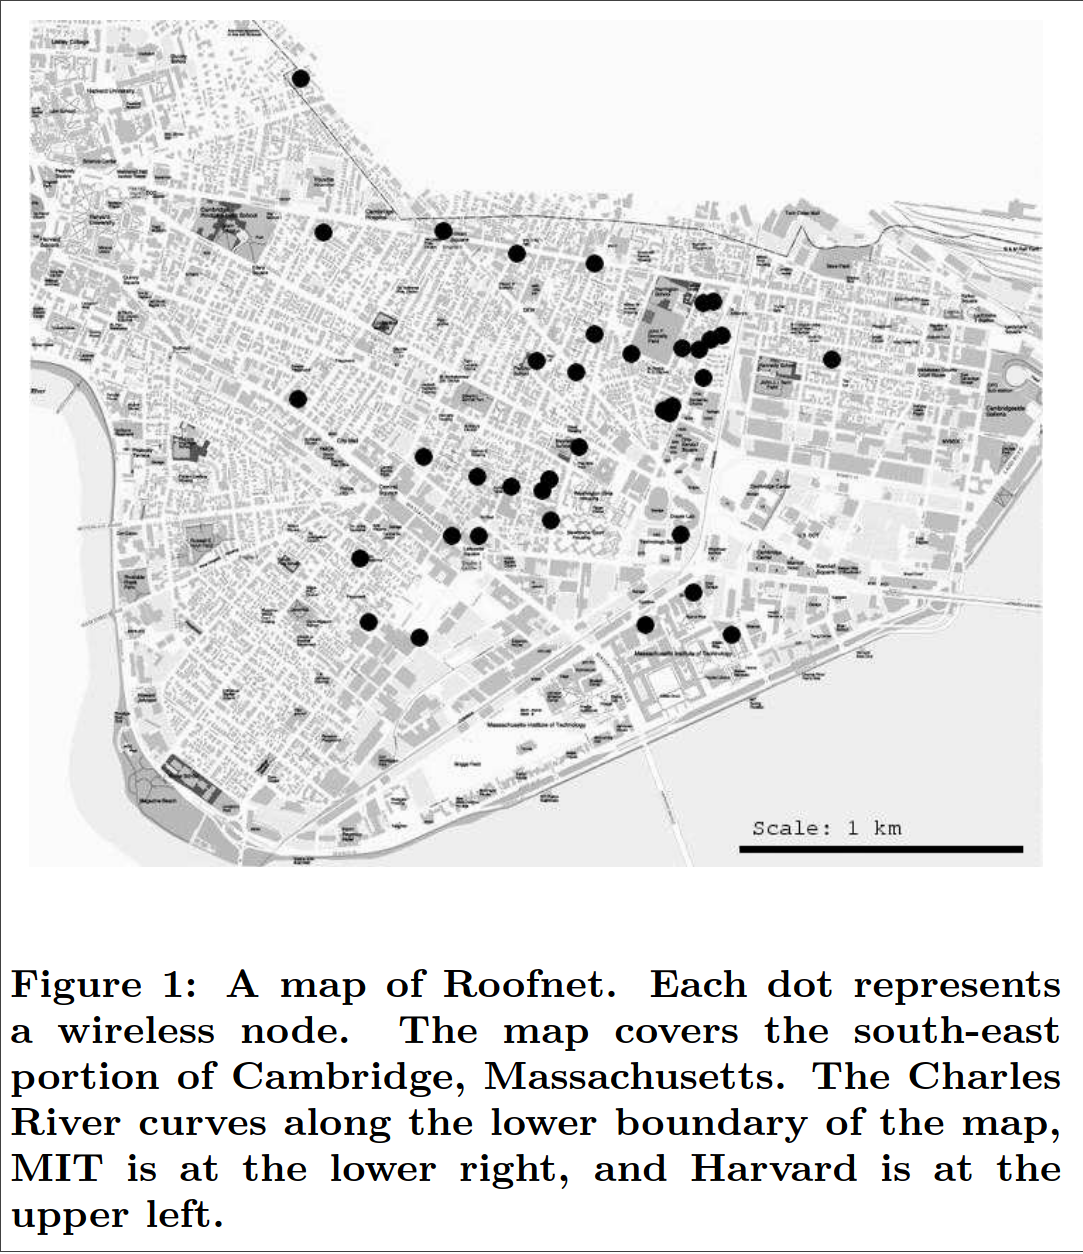
\includegraphics[height=0.8\textheight]{roofnet-fig1}
\end{frame}

\begin{frame}{roofnet routing}
    \begin{itemize}
    \item up to five hops for packet to get from one node to another
    \item link-state routing protocol between nodes
        \begin{itemize}
        \item no explicit configuration needed
        \end{itemize}
    \item sending nodes computed list of hops + included in packet
        \begin{itemize}
        \item idea called ``source routing''
        \item prevents transient routing loops
        \item important because conditions (e.g. weather) changes connectivity
        \end{itemize}
    \item everyone using same channel!
    \end{itemize}
\end{frame}

\begin{frame}{link-state/distance vector for wireless}
    \begin{itemize}
    \item no explicit list of links/networks
    \item instead: periodically broadcast and see who responds
    \item keep track of signal strength/reliabliy/etc. for routing metrics
    \end{itemize}
\end{frame}

\begin{frame}{modern mesh networks}
    \begin{itemize}
    \item common for distribution network between APs to be (partly) wireless
    \item sysadmin view:
        \begin{itemize}
        \item plug some APs into internet connection
        \item put other APs in appropriate place
        \item APs figure out how to make it work
        \end{itemize}
    \vspace{.5cm}
    \item typically using self-organizing mesh network ideas
        \begin{itemize}
        \item likely similar routing protocols to what we discussed
        \end{itemize}
    \item usually properietary networking protocols
        \begin{itemize}
        \item vendor lock-in problem
        \item (though there is now a recent Wifi standard)
        \end{itemize}
    \end{itemize}
\end{frame}




\section{centralized planning}
\begin{frame}{wifi polling mode}
    \begin{itemize}
    \item wifi has rarely used ``polling'' mode
    \vspace{.5cm}
    \item access point tells everyone when to transmit/not transmit
    \item periodically `poll' stations for more traffic
    \item can be mixed with periods allowing normal CSMA/CA
        \begin{itemize}
        \item carrier sense multiple access with collision avoidance
        \end{itemize}
    \vspace{.5cm}
    \item exercise: pro/con
    \end{itemize}
\end{frame}

\begin{frame}{deliberate scheduling}
\begin{itemize}
\item so far: 
    \begin{itemize}
    \item devices decide when to try to send or reply to requests
    \item one channel supporting one transmitter/receiver
    \end{itemize}
\vspace{.5cm}
\item alternate idea (cellular networks): divide
\item several available channels
    \begin{itemize}
    \item typically different frequencies
    \item signal encoding chosen to avoid interference between close frequencies
    \end{itemize}
\item slots within each time interval
\end{itemize}
\end{frame}

\begin{frame}

{\fontsize{9}{10}\selectfont Computer Networks: A Systems Approach, Figure 54}
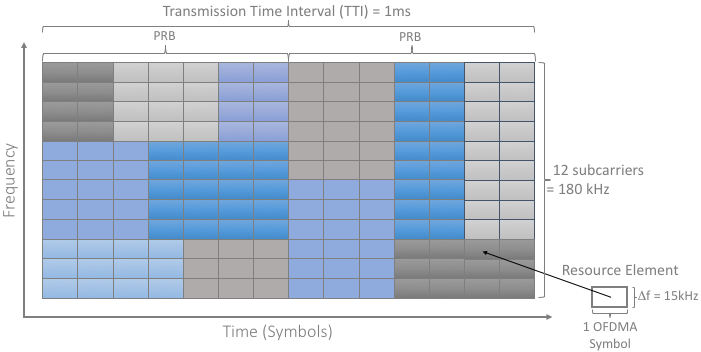
\includegraphics[width=\textwidth]{../multiaccess/CNSA-Fig54}
\end{frame}

\begin{frame}{central scheduler idea}
    \begin{itemize}
    \item `base stations' track active user devices
    \item users have bandwidth reservations
    \vspace{.5cm}
    \item base stations send out schedule of slots every $\sim$ 0.1--1ms
    \item protocol for handoff between base stations
    \item devices send back quality feedback to aid scheduling
    \end{itemize}
\end{frame}

\begin{frame}{dealing with propagation delay}
    \begin{itemize}
    \item schedule of slots will also have time delays
    \item goal: compensate for propogation delay
    \vspace{.5cm}
    \item base station needs to track estimate of propogation delay
    \end{itemize}
\end{frame}

\begin{frame}{dealing with new nodes}
    \begin{itemize}
    \item what about nodes without a reservation?
    \vspace{.5cm}
    \item mobile base stations advertise a `random access channel'
    \item used for reserving extra resources primarily
    \item use more wifi-like contention here
    \edn{itemize}
\end{frame}

\begin{frame}{exercise}
    \begin{itemize}
    \item central scheduling v carrier-sense
    \vspace{.5cm}
    \item exercise: which handles better\ldots
        \begin{itemize}
        \item utilizing the most of the available bandwidth
        \item independently controlled access points/base stations
        \item communications between two nearby nodes
        \end{itemize}
    \end{itemize}
\end{frame}


\section{firewall}

\begin{frame}[label=pktFilterExamples]{why packet filtering}
    \begin{itemize}
    \item some reasons to \textit{filter} packets:
    \vspace{.5cm}
    \item remove (malicious?) packets with false source addresses
    \item disallow external access to servers not on allowlist
    \item block traffic from known malicious sources
    \item only permit services on allowlist out of private network
    \end{itemize}
\end{frame}


\subsection{firewall: placement, state}
\begin{frame}{packet filters = firewalls}
    \begin{itemize}
    \item typical name for packet filter: ``firewall''
    \item especially filtering focused on security
    \end{itemize}
\end{frame}

\begin{frame}[label=ffDesign]<1>{firewall design decisions}
    \begin{itemize}
    \item where to filter?
        \begin{itemize}
        \item typically: \myemph<2>{at ``edges'' of network}
        \item in router, or separate box
        \item can also do elsewhere
        \end{itemize}
    \item how much to track when filtering?
        \begin{itemize}
        \item ``stateless'' or ``stateful''
        \end{itemize}
    \end{itemize}
\end{frame}

\againframe<2>{ffDesign}
\begin{frame}{the corporate firewall}
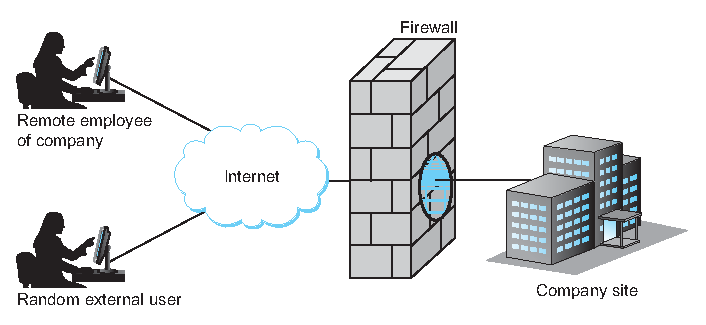
\includegraphics[width=0.9\textwidth]{sysapp-fig214}
\end{frame}



\subsection{zones of trust idea}
\begin{frame}{zones of trust}
    \begin{itemize}
    \item most common kind of firewall policy, three zones:
    \item internal network
        \begin{itemize}
        \item can send most things
        \item can't receive unsolicited traffic from external network
        \item where typical laptops/desktops live
        \end{itemize}
    \item DMZ (`demilitrized zone')
        \begin{itemize}
        \item not `protected' from external networks
        \item access to internal network similar to being within it
        \item where externally accessible services live
        \end{itemize}
    \item external network
        \begin{itemize}
        \item can only unsolicited to DMZ
        \item where the rest of the Internet lives
        \end{itemize}
    \end{itemize}
\end{frame}


\subsection{stateless firewall idea}
\begin{frame}{firewall rules}
    \begin{itemize}
    \item simple idea: look at packet's fields
    \item table indicating whether to reject
    \vspace{.5cm}
    \item similar idea to routing, but\ldots
    \item table matches fields other than destination
    \item table acitons are `drop', `reject', etc.
    \end{itemize}
\end{frame}


\begin{frame}{``stateless'' firewall}
    \begin{itemize}
    \item this design: table is set once by sysadmin
    \item doesn't change based on connections, etc.
        \begin{itemize}
        \item might change based on manual reconfiguration, etc.
        \end{itemize}
    \vspace{.5cm}
    \item called ``stateless''
    \vspace{.5cm}
    \item firewall doesn't track `state' based on current activity
    \end{itemize}
\end{frame}

\begin{frame}{exercise: what info do we need}
    \begin{itemize}
    \item what fields do we need to match these
        \begin{itemize}
        \item (and/or can we not handle without something more stateful?)
        \end{itemize}
    \vspace{.5cm}
    \item DNS queries to recursive DNS server from external servers
    \item packets with source address that does not match network
    \item packets from known malicious networks
    \item connecting from outside  to TCP servers not on allowlist
    \item connecting from inside using services (HTTP, etc.) not on allowlist
    \end{itemize}
\end{frame}


\subsection{nftables rules}
\begin{frame}[fragile]{Linux firewall: nftables}
\begin{itemize}
\item Linux's nftables --- one Linux kernel packet filter interface
    \begin{itemize}
    \item command-line tools + system call API implemented in kernel
    \item will show syntax for \texttt{nft} tool
    \item also some other kernel APIs: eBPF `programs', iptables
    \end{itemize}
\item different ``hooks'' where filtering can happen, list for IP:
    \begin{itemize}
    \item prerouting
    \item input (if received locally), forward (otherwise)
    \item output (if sent from local program)
    \item postrouting
    \end{itemize}
\item each hook has multiple ``chains'' of ``rules''
\end{itemize}
\end{frame}

\begin{frame}[fragile]{}
\begin{Verbatim}[fontsize=\fontsize{9}{10}\selectfont]
# for use with 'nft' on Linux; probably not the best way to write these rules:
table inet filter {
    chain EXTERNAL-INPUT {
        ip6 saddr {3fff:14::/32, 3fff:30::/32} drop
        ip saddr 198.51.100.0/24 drop
        ip6 daddr 3fff:14:1:15 tcp dport {80, 443} accept
        ip6 daddr 3fff:14:1::/48 tcp dport 22 accept
        drop
    }
    chain INTERNAL-INPUT {
        ip6 saddr != {3fff:14::/32, 3fff:30::/32} drop
        ip saddr != 198.51.100.0/24 drop
        udp dport 137 drop
        accept
    }
    chain INPUT {
        type filter hook input priority 0
        iifname lo accept
        iifname ethExt jump EXTERNAL-INPUT
        iifname ethInt jump INTERNAL-INPUT
        reject
    }
}
\end{Verbatim}
\end{frame}



\subsection{things we can't do}
\begin{frame}{limits of packet matching?}
    \begin{itemize}
    \item so far: showing stateless filtering
    \vspace{.5cm}
    \item can stateless filtering to do a lot\ldots:
    \item match more header fields
    \item check if packet contents match pattern
    \vspace{.5cm}
    \item but some fundamental limits of design
    \end{itemize}
\end{frame}

\begin{frame}[fragile]{filtering connections? (1)}
    \begin{itemize}
    \item let's say we're writing rule on router between 3fff::/16 network
    and internet
    \item want to rule allow\ldots
    \item TCP connections from 3fff::2 to outside machines
    \item and drop all other traffic
    \vspace{.5cm}
    \item can't really do this with stateless rules
    \item but can come close
    \end{itemize}
\end{frame}

\begin{frame}[fragile]{exercise (1)}
\begin{itemize}
\item goal: allow 3fff::2 outside TCP connections only
\item how is this going to break?
    \begin{itemize}
    \item assume we run this only packets about to be forwarded in router
    \end{itemize}
\end{itemize}
\begin{Verbatim}[fontsize=\fontsize{9}{10}]
ip6 saddr 3fff::2 protocol tcp accept
drop
\end{Verbatim}
\end{frame}

\begin{frame}[fragile]{exercise}
\begin{itemize}
\item goal: allow 3fff::2 outside TCP connections only
\item assume \texttt{ethInt} = inside; \texttt{ethExt} = outside
\item is this good enough?
    \begin{itemize}
    \item assume we run this only packets about to be forwarded in router
    \end{itemize}
\end{itemize}
\begin{Verbatim}[fontsize=\fontsize{9}{10}]
iifname ethInt protocol tcp accept
iifname ethExt protocol tcp flags & (fin|syn|rst||ack) == syn drop
iifname ethExt ip6 daddr 3fff::2 protocol tcp accept
iifname ethExt ip6 daddr 3fff::2 icmpv6 { destination-unreachavble, time-exceeded } accept
drop
\end{Verbatim}
\end{frame}



\section{stateful firewalls}

\subsection{connection tracking}

\subsubsection{what about UDP}

\subsubsection{PING/PONG; TCP keepalive}

\subsubsection{extra connections in FTP, IRC, etc}

\section{NAT traversal}

\subsection{discovering external addresses}

\subsection{via connection state manipulation}

\subsection{UPnP}

\subsection{TURN}

\section{IDSes}

\subsection{snort}

\section{network address translation}

\subsection{motivation: missing addresses}

\subsection{reusing connection tracking}


\section{backup slides}
\begin{frame}{backup slides}
\end{frame}

\end{document}
